
%%% 将整型数据类型时讲解%%%%%%%%%%%%%%%%


\begin{frame}{实型十进制数转换为二进制数}
分别转换整数部分和小数部分。 整数部分: 除2取余, 至商为0, 逆序排列余数, 得到整数部分的二进制位。小数部分, 乘2取整, 至小数部分为0或指定精度, 正序排列, 即得小数部分的二进制位。
\begin{align*}
(11.625)_{10}&=1\times 2^3+0\times 2^2+1\times 2^1+1\times 2^0+1\times 2^{-1}+0\times 2^{-2}+1\times 2^{-3}\\
&=(1011.101)_2
\end{align*}

\begin{center}
\opmul[voperator=bottom,carryadd=false]{0.625}{2}\qquad\qquad \opmul[voperator=bottom,carryadd=false]{0.25}{2}\qquad\qquad \opmul[voperator=bottom,carryadd=false]{0.5}{2}
	
正序排列各整数得到小数部分的二进制位$(101)_2$
\end{center}
	
\color{blue}{$(0.101)_2=1\times 2^{-1}+0\times 2^{-2}+1\times 2^{-3}=0.625$}
\end{frame}

\begin{frame}[shrink]{例: 把0.5773转换成二进制(保留到小数点后7位)。}
\colorbox{yellow}{注: 用二进制表示小数部分有精度问题。}
\begin{align*}
&                      &&\text{积的整数部分}\\
&0.5773\times 2=1.1546 && 1\\
&0.1546\times 2=0.3092 && 0\\
&0.3092\times 2=0.6184 && 0\\
&0.6184\times 2=1.2368 && 1\\
&0.2368\times 2=0.4736 && 0\\
&0.4736\times 2=0.9472 && 0\\
&0.9472\times 2=1.8944 && 1
\end{align*}
\begin{align*}
(0.1001001)_2&=1\times 2^{-1}+0\times 2^{-2}+0\times 2^{-3}+1\times 2^{-4}+0\times 2^{-5}+0\times 2^{-6}+1\times 2^{-7}\\
&=0.5703125\ne 0.5773   
\end{align*}
\end{frame}

\begin{frame}[shrink]{数值在计算机中的表示(以8bit编码为例)}
\begin{itemize}
	\item 原码:正数的符号为0,负数的符号为1,其它位按一般的方法表示数的绝对值。
	\vspace{-0.5cm}
	\begin{align*}
	x=(+103)_{10}  &&[x]_{\text{原}}=(\textcolor{red}{0}1100111)_{2}\\
	x=(-103)_{10}  &&[x]_{\text{原}}=(\textcolor{red}{1}1100111)_{2}
	\end{align*}
	\item 反码: 正数的反码与原码相同;负数的反码是符号位不变,其他位按位取反 
	\item 补码: 正数的补码与其原码相同;负数的补码为其反码最末位加1. 即,
	
	 \textcolor{blue}{负数补码 = 反码$+1=2^n-$该数的绝对值, $n$是编码二进制位数.}
\end{itemize}
\vspace{-0.5cm}
\begin{align*}
(77)_{10}&=(\textcolor{red}{0}100\quad 1101)_{2},\qquad (-77)_{10}=(\textcolor{red}{1}100\quad 1101)_{2}\\
(-77)_{\text{补}}=2^8-77&=\textcolor{red}{1}111\quad 1111 +\textcolor{red}{0}000\quad 0001 - \textcolor{red}{0}100\quad 1101\\
&=\underbrace{\textcolor{red}{1}111\quad 1111 - \textcolor{red}{0}100\quad 1101}_{(-77)_{\text{反}}} + ~\textcolor{red}{0}000\quad 0001\\
&=\underbrace{\textcolor{red}{1}011\quad 0010 }_{(-77)_{\text{反}}}+ \textcolor{red}{0}000\quad 0001=1011\quad 0011
\end{align*}
\end{frame}

\begin{frame}{数值表示示例}
\centering
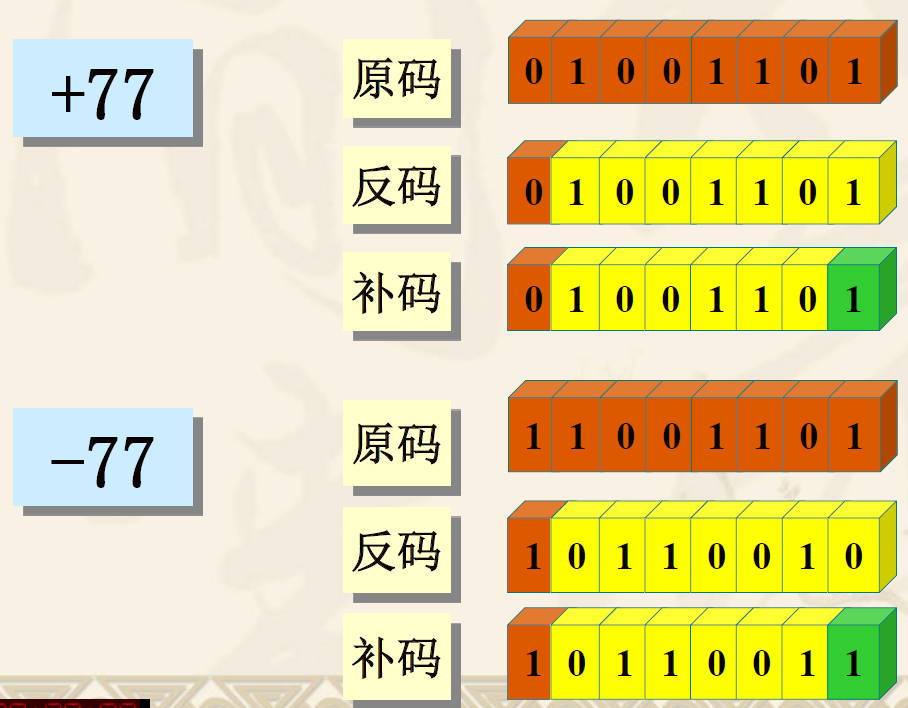
\includegraphics[scale=0.25]{2}
\end{frame}

\begin{frame}{机内以补码形式存储有符号数}
\begin{enumerate}
	\setlength{\itemsep}{.5cm}
	\item 对于正数,原码=反码=补码
	\item 对于负数,补码=反码 + 1\\
	      反码 = 符号位不变, 其他位按位取反
	\item 补码是可逆的,即再对补码求补得到原码。
	\item 引入补码后,使减法统一为加法。
	$(+77)_{\text{补}}+(-77)_{\text{补}}=0100~1101+1011~0011=0000~0000$	
\end{enumerate}
\end{frame}

\note
{
	0原码是00000000 -0原码是10000000
	
	0反码是00000000 -0反码是11111111
	
	0补码是00000000 补码没有正0与负0之分。+0和-0的补码是一样的。即 0的补码只有一种表示。
	
	+0的补码:00000000
	
	-0的补码:第一步:11111111 第二步+1= 1 00000000 第三部:进位1被丢弃 您明白了吗?
	
	在规定中,8位二进制码能表示的反码范围是-127~127。
	
	此时(字长为8位), -128没有原码和反码(只有补码)。
	
	那么,为什么规定字长8位时-128没有原码和反码呢?下面解释。
	
	首先看-0,[-0]原码=1000 000,其中1是符号位,求反操作,算出[-0]反码=1111 1111,
	
	再看-128,假如它有原码且[-128]原码=1000~000,假如让-128也有反码,求反操作,则[-128]反码=1111~1111,
	
	你会发现,-128的反码和-0的反码相同,所以为了避免面混淆,有了-0的原码,便不能有-128的原码补码,这是8位比特位位数限制决定的。
}

\begin{frame}{补码运算实例(以8bit编码为例)}
\textcolor{blue}{补码可逆:}
\begin{align*}
&[-25]_{\text{原}}=(1001~1001)_2\quad [-25]_{\text{反}}=(1110~0110)_2\\
&[-25]_{\text{补}}=[-25]_{\text{反}}+1=(1110~0110+1)_2=(1110~0111)_2\\
&[-25]_{\text{原}}=\left([-25]_{\text{补}}\right)_{\text{补}}=(1001~1000+1)_2=(1001~1001)_2
\end{align*}

\textcolor{blue}{减法统一为加法: $[a-b]_{\text{补}}=a_{\text{补}}+[-b]_{\text{补}}$}
\begin{align*}
&[102-25]_{\text{补}}=[77]_{\text{补}}=(0100~1101)_2=77\\
&[102]_{\text{补}}+[-25]_{\text{补}}=(0110~0110)_2+(1110~0111)_2=(0100~1101)_2=77\\
&\text{所以, }[102-25]_{\text{补}}=[102]_{\text{补}}+[-25]_{\text{补}}\\
&\text{同样有, }[25-102]_{\text{补}}=[25]_{\text{补}}+[-102]_{\text{补}}\\
\end{align*}
\end{frame}

\begin{frame}{ASCII编码表$B_6B_5B_4B_3B_2B_1B_0$}
\begin{columns}
	\column{0.65\textwidth}
	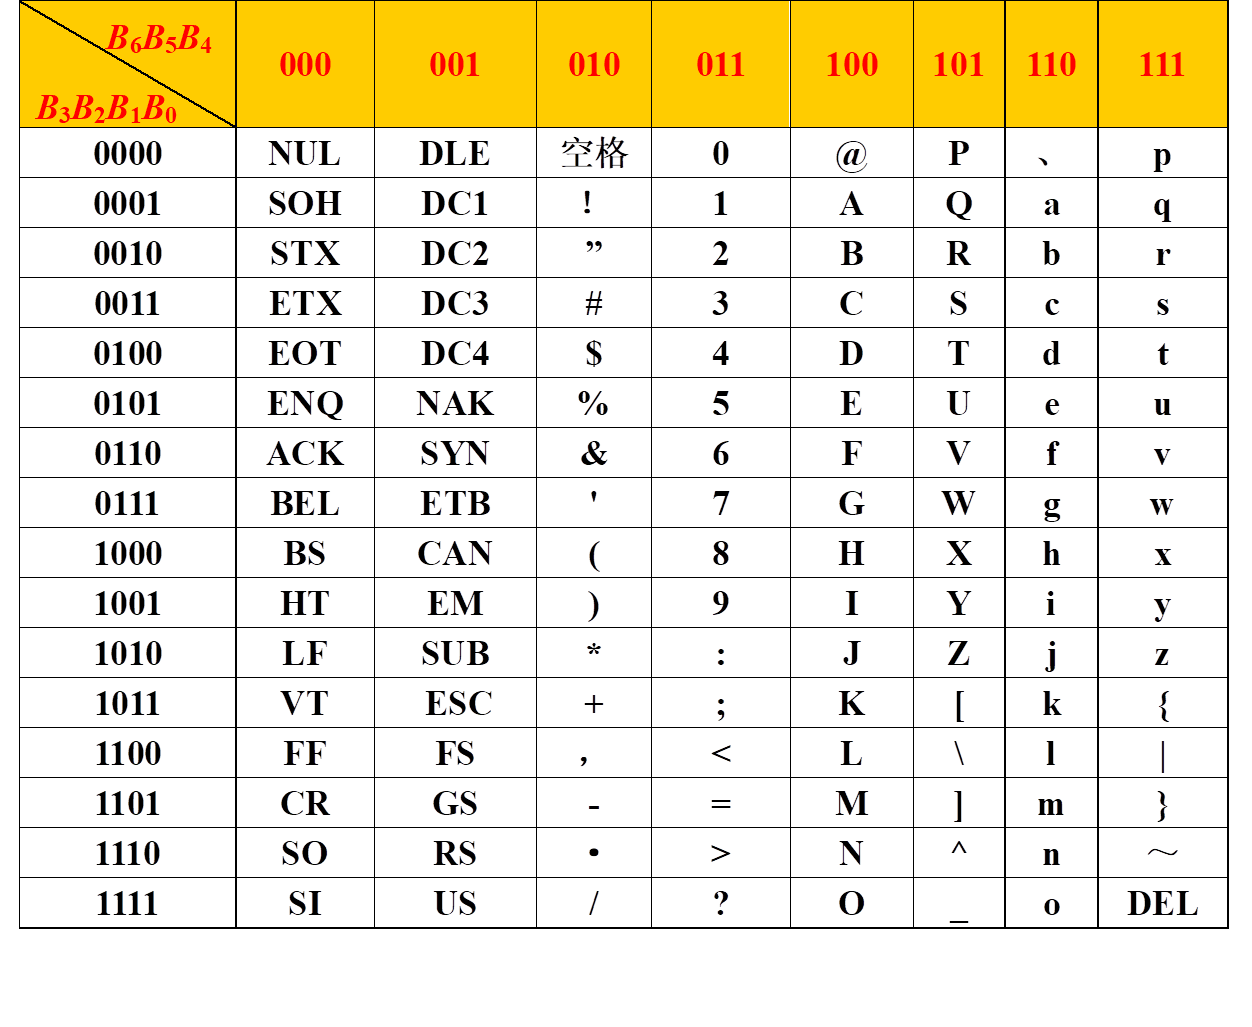
\includegraphics[scale=0.4]{ASCII}
	\column{0.35\textwidth}
	\begin{itemize}
		\item ASCII码连续排列 \\
		 `0'$\sim$`9', `A'$\sim$`Z', `a'$\sim$`z'
		\item 数字 = 编码值 - `0' \\
		 9=`9'-`0'
		\item 大小字符间隔: \\
		`a' - `A' = 32
		
		\scriptsize{
		`a'=0110~0001=61H=0X61=97
		
		'A'=0100~0001=41H=0X41=65}
	\end{itemize}	
\end{columns}
\end{frame}

%%%%%%%%%% 线上讲解这部分内容 %%%%%%%%%%%%%%%%%%%%

\section{Algorithm + Data Structures = Programs}

\begin{frame}{数据结构与算法}
\begin{columns}
	\column{0.4\textwidth}
	\begin{block}{}
		算法 + 数据结构 = 程序\\
		Algorithm + Data Structures = Programs
	\end{block}
	%\hspace{20pt}
	\column{0.4\textwidth}
	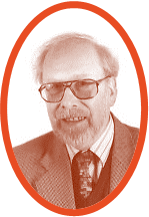
\includegraphics[scale=0.4]{Wirth}\\
	沃思(Niklaus Wirth)
\end{columns}
\begin{itemize}
	\item 数据结构\\
	对数据的描述。在程序中要指定用到哪些数据,以及这些数据的类型和数据的组织形式。
	\item 	算法\\
	对操作的描述。即要求计算机进行操作的步骤	
\end{itemize}
\end{frame}

\begin{frame}{程序员的工作}
\centering
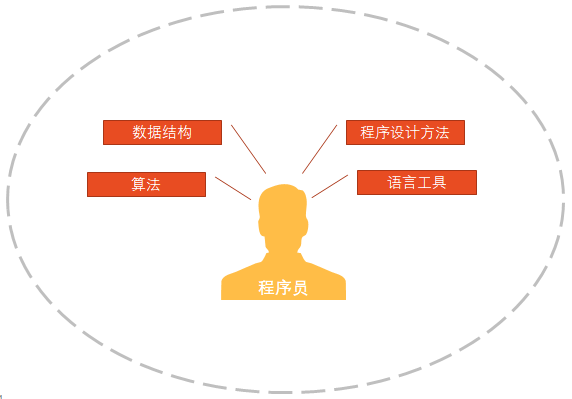
\includegraphics[scale=0.5]{programer}
\end{frame}

\begin{frame}{算法}
\begin{columns}
\column{0.4\textwidth}

\includegraphics[scale=0.25]{programer2}
\column{0.5\textwidth}
\begin{block}{算法}
\begin{itemize}
	\item 广义地说,为解决一个问题而采取的方法和步骤,就称为“算法”。
	\item 对同一个问题,可以有不同的解题方法和步骤。
	\item 为了有效地进行解题,不仅需要保证算法正确,还要考虑算法的质量,选择合适的算法。
\end{itemize} 
\end{block}
\end{columns}
\end{frame}

\begin{frame}{算法}
\begin{columns}[t]
\column{0.45\textwidth}
\begin{block}{数值运算算法}
如求一个方程的根, 计算一个函数的定积分等。\\
数值运算的目的是求数值解。\\
由于数值运算往往有现成的模型,可以运用数值分析方法,因此对数值运算的算法的研究比较深入,算法比较成熟。	
\end{block}
\column{0.45\textwidth}
\begin{block}{非数值运算算法}
如图书检索, 人事管理等。\\
计算机在非数值运算方面的应用远超在数值运算方面的应用。
非数值运算的种类繁多,要求各异,需要使用者参考已有的类似算法,重新设计解决特定问题的专门算法。
\end{block}
\end{columns}
\end{frame}

\begin{frame}[shrink]{简单的算法举例[例2.1(p17)]}
\begin{example}
[例2.1(p17)] 求$1\times 2\times 3\times 4\times 5$
\end{example}
\vspace{-0.7cm}
\small
\begin{columns}[t]
\column{0.45\textwidth}
\begin{block}{算法(一)步骤}<1->
\begin{enumerate}
\item[S1] 先求1乘以2,得到结果2
\item[S2] 将步骤1得到的乘积2再乘以3,得到结果6
\item[S3] 将6再乘以4,得24
\item[S4] 将24再乘以5,得120
\end{enumerate}	
\end{block}
\begin{block}{思考}<3->
求$1\times 3\times 5\times 7\times 9$
\end{block}
\column{0.45\textwidth}<2->
\begin{block}{算法(二)步骤}
\begin{enumerate}
\item[S1] $p=1$, 表示将1存放在变量p中
\item[S2] $i=2$, 表示将2存放在变量i中
\item[S3] $p=p*i$, 使p与i相乘,乘积仍放在变量p中
\item[S4] $i=i+1$, 使变量i的值加1
\item[S5] if (i<=5) goto S3\\
else 算法结束, 最后得到p的值就是5!的值。
\end{enumerate}	
\end{block}
\end{columns}
\end{frame}

\begin{frame}[shrink]{简单的算法举例[例2.2(p18)]}
\begin{example}
[例2.2(p18)] 有50个学生,要求输出成绩在80分以上的学生的学号和成绩.
\end{example}

\begin{block}{算法步骤}<2->
float g[50]=\{100,90.5,30.8,$\cdots$\}; \textcolor{red}{// 表示50名学生成绩}\\
int i = 0;  \textcolor{red}{//表示第i个学生学号}\\
while(i<50) \\
\{ \\
\qquad if (g[i]>=80) printf("第\%d个学生成绩\%f, " , i+1, g[i]); \\
\qquad i = i + 1;\\
\} 
\end{block}
\end{frame}

\begin{frame}{例2.3(p18): 闰年判定条件.}
\centering
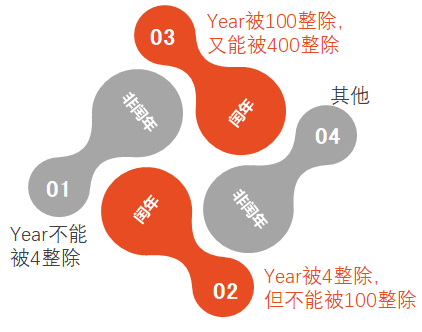
\includegraphics[scale=0.4]{leap}
\end{frame}

\note{
1、普通闰年:公历年份是4的倍数的,一般是闰年。(如2004年就是闰年);

2、世纪闰年: 公历年份是整百数的,必须是400的倍数才是闰年(如1900年不是世纪闰年,2000年是世纪闰年)。
}

\begin{frame}[shrink]
\begin{columns}%[T] % align columns
\begin{column}{1.0\textwidth}
\begin{algorithm}[H]  
\caption{例2.3(p18): 判定2000—2500年中的每一年是否为闰年.} %算法的名字
\begin{algorithmic}[1] %每行显示行号
\State int year=2000, char R; \textcolor{red}{// R是标志变量, 'Y'或'N'}
\While{(year<=2500)} % While语句,需要和EndWhile对应
\State R=`N';  
\If{(year能被4整除,但是不能被100整除)} R=`Y'; % If 语句,需要和EndIf对应
\ElsIf {(year能被100整除, 并且能被400整除)} R=`Y';
\EndIf
\If{(R=='Y')} printf(``\%d是闰年", year); 
\Else \quad printf(``\%d不是闰年", year);
\EndIf	
\State year = year + 1;
\EndWhile
\end{algorithmic}  
\end{algorithm}
\end{column}%
\end{columns}


\begin{frame}%[shrink]
\begin{columns}%[T] % align columns
\begin{column}<0->{.8\textwidth}
%\scriptsize
\begin{algorithm}[H]  
\caption{例2.4(p19): 求$1-\frac{1}{2}+\frac{1}{3}-\frac{1}{4}+\cdots+\frac{1}{99}-\frac{1}{100}$.} %算法的名字
\begin{algorithmic}[1] %每行显示行号
\State int sign=1, deno=2;
\State float sum = 1.0; 
\While{(deno<=100)} % While语句,需要和EndWhile对应
\State sign = -1 * sign;
\State sum = sum + sign*1.0/deno; 
\State deno = deno + 1; 
\EndWhile
\State printf(``sum=\%f$\backslash$n", sum);	
\end{algorithmic}  
\end{algorithm}
\end{column}%
%\hfill%	
\begin{column}<0->{.20\textwidth}
\newline
\newline
sign: 表示当前项的数值符号\\
deno: 表示当前项的分母\\
sum:  表示当前项的累加和
\end{column}%
\end{columns}
\medskip
\colorbox{green}{问题: 为何使用sign*1.0 ?}
\end{frame}

\begin{frame}%[shrink]
\begin{columns}%[T] % align columns
\begin{column}<0->{1.0\textwidth}
%\scriptsize
\begin{algorithm}[H]  
\caption{例2.5(p20): 给出一个大于或等于3的正整数,判断它是不是一个素数.} %算法的名字
\begin{algorithmic}[1] %每行显示行号
\State int n, i=2;
\State scanf("\%d",\&n); \textcolor{red}{// 输入n的值.} 
\While{(i < n)} % While语句,需要和EndWhile对应
\If{(n能被i整除)} \{ printf(``\%d不是素数", n); return; \}
\EndIf
\State i = i + 1;
\EndWhile
\State printf(``\%d是素数", n);	
\end{algorithmic}  
\end{algorithm}
\end{column}%
%\hfill%	
\end{columns}
\begin{block}{Notes}
实际上, $n$不必检查被$2\sim(n-1)$之间的整数整除, 只须检查能否被$2\sim\sqrt{2}$间的整数整除即可。
\end{block}
\end{frame}

\begin{frame}{算法的特性}
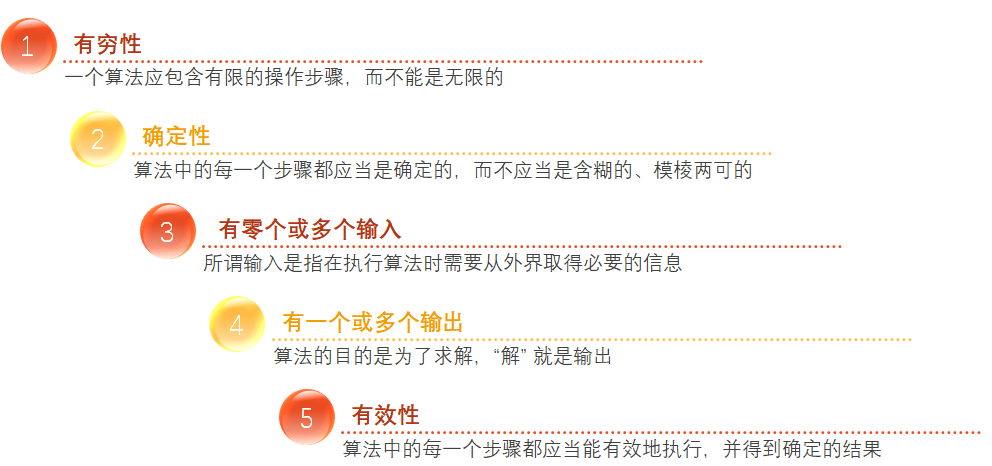
\includegraphics[scale=0.35]{algo}
\end{frame}

\begin{frame}{结构化程序设计方法}
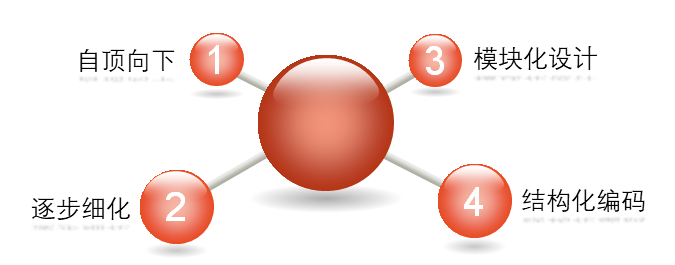
\includegraphics[scale=0.5]{top-down}
\end{frame}
%%%%%%%%%%%%%%%%%%%%%%%%%%%%%%%%%%%%%


% 讲条件语句时讲解

\begin{frame}[fragile]{if(条件表达式)\{ 表达式为真(非0)时执行语句; \}}
\begin{lstlisting}
#include<stdio.h>            // standard input/output编译预处理指令
int main()                   // 主函数
{                            // 函数开始标志
int a=10;    // 定义变量a为整型数值, 定义变量时,可以指定变量的初值
if(a>=10)
{
printf("a>=10\n"); // \n为换行符
}
else
{
printf("a<10\n"); // \n为换行符
}
return 0;                 // 函数执行完毕返回函数值0
}                            // 函数结束标志
\end{lstlisting}
\end{frame}

\begin{frame}[fragile]{while(条件表达式)\{ 表达式为真(非0)时执行的语句;\}}
\begin{lstlisting}
#include<stdio.h>            // standard input/output编译预处理指令
int main()                   // 主函数
{                            // 函数开始标志
int a=10;    // 定义变量a为整型数值, 定义变量时,可以指定变量的初值
while(a>=0)
{
printf("a=%d\n",a); // \n为换行符
a--; // a= a - 1
}
return 0;                 // 函数执行完毕返回函数值0
}                            // 函数结束标志
\end{lstlisting}
\end{frame}
%%%%%%%%%%%%%%%%%%%

